%%%%%%%%%%%%%%%%%%%%%%%%%%%%%%%%%%%%%%%%%%%%%%%%%%%%%%%%%%%%%%%%%%%%%%%%%%%%%%%%
\chapter{Conclusion and Future Work}\label{ch:conclusion}
%%%%%%%%%%%%%%%%%%%%%%%%%%%%%%%%%%%%%%%%%%%%%%%%%%%%%%%%%%%%%%%%%%%%%%%%%%%%%%%%





\section{Future Work}

In this section we discuss some ideas for future works and implementation for SIMITAR. We suggest approaches to get better results. They include perfromance improovments, calibration of some constants and finer controll of packet injection. We list them as a task list in the talbe  


\begin{table}[ht!]
	\centering
	\caption{Future Work: task list}
	\label{tab:task-list}
	\begin{tabular}{cccc}
		\hline
		\multicolumn{3}{c}{{\color[HTML]{000000} Future Work}}                                                                               & Priority                \\ \hline
		1                      & Optimizing linear regression                              &                                                 & \textit{high}                    \\
		2                      & Flow-merging option                                       &                                                 & medium                  \\
		3                      & Smart flow-scheduler                                      &                                                 & \textit{high}                    \\
		4                      & \texttt{DataProcessor::minimumAmountOfPackets}                         &                                                 & low                     \\
		5                      & DPDK KNI interfaces                                       &                                                 & low                     \\
		6                      & Multi-thread C++ sniffer                                  & \multirow{-6}{*}{Performance}                   & \textit{high}                    \\ \hline
		7                      & Model inter-packet times on \texttt{TinsFlow}           &                                                 & \textit{high}                    \\
		8                      & D-ITG flow generator (\texttt{DitgFlow})                &                                                 & low                     \\
		9                      & DPDK flow generator (\texttt{DpdkFlow})                 &                                                 & medium                     \\
		10                     & Ostinato flow generator (\texttt{OstinatoFlow})         & \multirow{-4}{*}{Tool support}                  & low                     \\ \hline
		11                     & \texttt{DataProcessor::min\_time}                       &                                                 & low                     \\
		12                     & \texttt{DataProcessor::m\_min\_on\_time}                &                                                 & low                     \\
		13                     & \texttt{DataProcessor::m\_session\_cut\_time}           &                                                 & low                     \\
		14                     & Minimum number of packets per flow option                 & \multirow{-4}{*}{Calibration}  & low                     \\ \hline
		15 & Python API/Lua for traffic generation & & low \\
		16 & Crafter of  pcap files & & low \\
		%17 & Json compact trace descriptor  & \multirow{-3}{*}{New features} & low 
		\hline
	\end{tabular}
\end{table}





(1) The major issue of SIMITAR now is optimizing data processing for creating the compact trace descriptor. The performance becomes an issue when processing large \textit{pcap} files with more dozens of thousands of flows. The processing in this case may take some hours. In the current implementation, the linear regression is mono-thread, and the stop criteria are just the number of iterations. Parallel processing, and creating stop criteria based on convergence, alongside with the number of iterations, should increase the processing performance. 

(2) Crating an option for merging flows is a possibility to imprrove performance of traffic with several thousands of flows and Gigabits of bandwidth, such as from WAN captures. A merge criterion for example is considere just network headers to classify the flows. 

(3) On the traffic generation, currently, the threads for all flows are being instantiated once the traffic generations start. A smarter traffic generation, where each thread is instantiated when the traffic is active and dies when it is inactive should reduce the overhead for \textit{pcap} files with a large number of flows. For traffic with a massive amount of flows, a methodology for merging them should reduce overheads and enable replication of traffic with a much larger bandwidth. 


(4) Constant \texttt{DataProcessor::minimumAmountOfPackets}: SIMITAR only estimates stochastic models for inter-packet times if the number of flow packets is larger than this value. If it is smaller, we use only the constant model, for two reasons. First, because with a small sample, the accuracy estimate stochastic model is poor. Second, because we avoid the parameterization process, which is cost in the case of linear regression. Its value today is set to 30. Increasing this value, we may achieve a more reasonable performance for individual flows, and reduce the processing time. 


(5) One possibility to improove the traffic generation performance isuse DPDK KNI interfaces \footnote{\href{http://dpdk.org/doc/guides/prog_guide/kernel_nic_interface.html}{http://dpdk.org/doc/guides/prog\_guide/kernel\_nic\_interface.html}}. The The DPDK Kernel NIC Interface (KNI) allow applications from the user's space interact with DPDK ports. In this way, we may achieve a faster packet processing. This can be integrated as an instatiatable feature of SIMITAR (figure ~\ref{fig:dpdk-if}).


\begin{figure}[h!]
	\centering
	\subfloat[DpdkFlow]{
		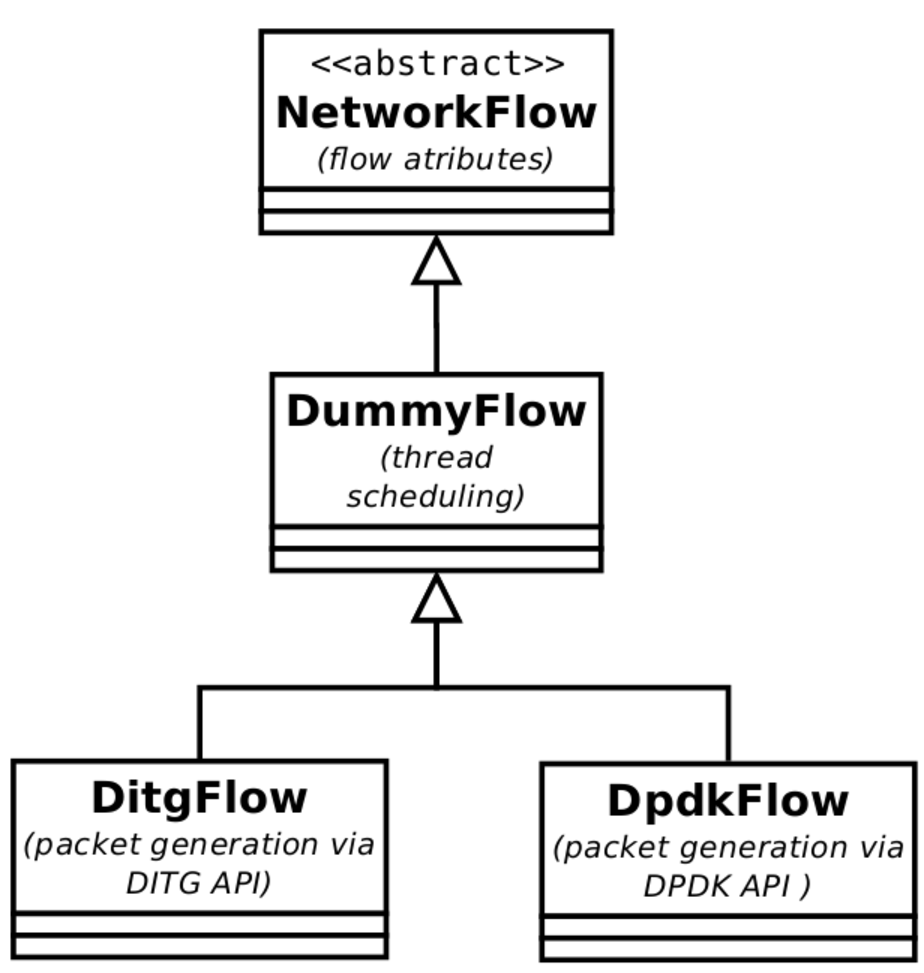
\includegraphics[height=2.0in]{figures/ch6/dpdk-flow}
		\label{fig:dpdk-flow}
	}
	\hspace{0mm}
	\subfloat[DpdkInterface]{
		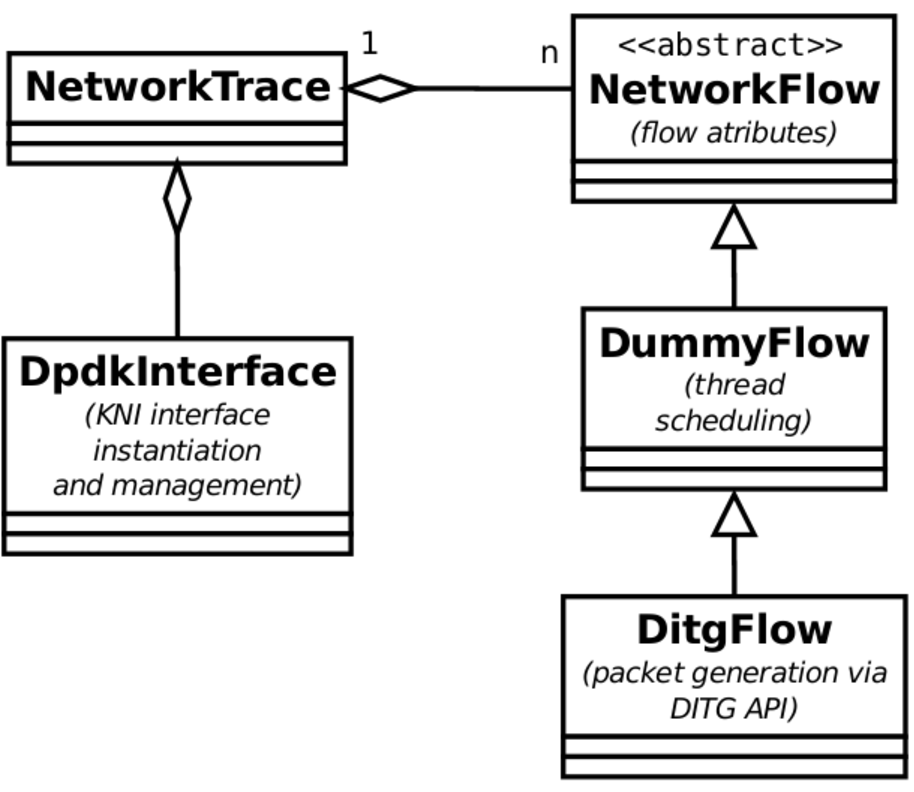
\includegraphics[height=2.0in]{figures/ch6/dpdk-interface}
		\label{fig:dpdk-if}
	}
	\caption{Class diagram for DPDK support expansions. On (a), we have a implementation of traffic generation based on DPDK. On (b) we are using DPDK KNI interfaces.}
	\label{fig:DpdkFlow}
\end{figure}


(6) Another issue is the sniffer component is taking to much time to extract data form large \textit{pcap} files. Implementing an C/C++ multi-thread sniffer, includding the packet processing and the SQL queries, will improove its performance. 


(7) SIMITAR's current implementation using \textit{libtins} to generate the packets does not model inter-packet times. To avoid processing overheads on calculating random numbers, these values may be calculated before the actual traffic generation, and then be used. By this approach, the scaling characteristics of the traffic generated by libtins should improve, and be closer to the original traffic. 

(8-10) Expand SIMITAR to other traffic generator tools, as we present in the figure ~\ref{fig:DpdkFlow}. D-ITG offers many stochastic functions for cusmtumization of inter-packet times, Ostinato offers a rich header and protocol custumization, and DPDK a high performance on packet generation. Each tools is able to affer a different result on traffic generation, each with benefits and drawbacks, such as cumputation cost, and complexity of development. DPDK offers the possibility to bypass the Linux network stack, called packet acceleration. So, this implementation could enable for SIMITAR high-bandwidht along wiht traffic realism.

(11) Constant \texttt{DataProcessor::min\_time}: smallest time considered for inter-packet times. We use this value to avoid inter-packet times equals to zero due to the sniffer resolution. In that case, some of our procedures would diverge. It can change the fitting accuracy. Today, this value is $5e-8$.


(12) \texttt{DataProcessor::m\_min\_on\_time}: this value controls the small ON time that a \textit{file} can have. This value  can change the precision of the generated traffic. Currently this value is $0.1$s. 


(13) Constant \texttt{DataProcessor::m\_session\_cut\_time}: this member defines whatever a file transference still active or has ended. It defines the smallest OFF time acceptable. This value will change how many files SIMITAR will transfer per flow, and how many times it will call the underlying traffic generator. This constant may affect both computational performance and traffic realism.


(14) Constant \textit{Control a minimum number of packets required for SIMITAR create a new flow}: This would reduce the number of flows created, improving its computational performance. Since SIMITAR manages each flow in a  different thread, it will create fewer threads, reducing overheads. This action should not impact  on throughput and scaling characteristics because few packets would be ignored. But it can increase the precision of the most significant flows since all the threads are competing each other on the Operational System. But, the number of flows created would be smaller.


(15) Currently, SIMITAR only enables the programming of flow traffic generation in C++. Adding Python and Lua support for reading NetwrokTrace and NetworkFlow objects, we can enable expansion for Python/Lua traffic generation APIs (such as Ostinato and MoonGen APIs), without creating C++ "wrappers".


(16) \textbf{PcapGen: a compact \textit{pcap} lybrary}: Create a component capable of generate synthetic \textit{pcap} files, using Compact Trace Descriptors(CTDs) files. We can implement this using SIMITAR as a packet injector, but in an emulated host interface, for example, using Mininet. Then, the traffic can be collected, using a tool such as TCPDump or Tshark. We present a diagram of this idea in the figure ~\ref{fig:pcap-gen}. This expansion would enable SIMITAR  to work as trace library for pcap-based benchmark tools.

\begin{figure}[!ht]
	\centering
	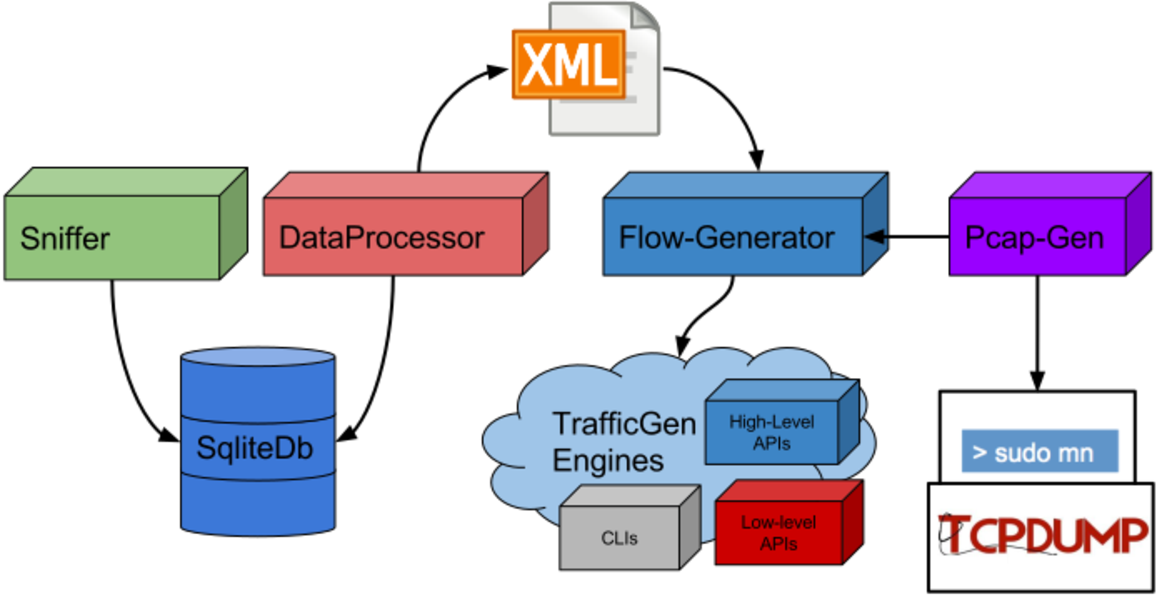
\includegraphics[height=2.0in]{figures/ch6/pcap-gen}
	\caption{Using SIMITAR for generation synthetic \textit{pcap} files, CTD files: a component schema}
	\label{fig:pcap-gen}
\end{figure}
	


%\item \textbf{Use OpenDayLight REST API for data collection}: Another different approach for data collection could be the use the OpenDayLight REST API to collect data from an SDN OpenFlow switches, instead of a using a Sniffer. Through REST API is possible to extract many statistics from nodes, hosts, and ports, such active flows, the number of packets matched per flows, packet drops, and so on. But, different features would be measured,  and a new model for traffic generation would be needed. On the other hand, we could reuse many procedures implemented.  

%\subsection{Changing the Model, reusing the Architecture}

%Since the proposed architecture is model-independent, another future work is to use the same general concepts of compact trace descriptor and API agnostic modeling on different models and compare the results.

%Our proposed future work is to implement this idea using the Swing\cite{swing-paper} and the Harpoon Model\cite{harpoon-paper}.  We can create not just Simitar trace descriptors, but Swing and Harpoon trace descriptors as well. So, as here, we would have the same components: the Sniffer, the SQLite database, the DataProcessor, the flow generator, and the same interface based on an XML Compact Trace Descriptor. The FlowGenerator would abstract the traffic generation in based on the Swing and Harpoon model, in an API independent way as well. 

%These implementations can lead to a definitive and standardized model of realistic traffic generation. In this way, progresses on high-speed traffic generation would no more make old traffic generators and models obsolete. Also, would enable the comparison (ain a fair way) which model is actually the best since the same engine and technic for generating packets will be used.

%Also, the idea of a Compact Trace Descriptor, by itself separates the idea of traffic generation and the modeling. De development of new methodologies for modeling is  separated from the traffic generation. So a data-developer, using any compact trace descriptor interface may just "plug" his method of data modeling in the FlowGenerator. He has not to care about how the packets were going to be generated anymore nor in what programming language is being used to craft packets.


\section{Final Conclusions}





TODO considerações, contrubuições, lições, boas idéias, mas idéias



\textcolor{red}{some text here}







